% C.12 等边三角形边长4
\documentclass[tikz,border=4pt]{standalone}
\usepackage{ctex}
\usepackage{amsmath}
\usetikzlibrary{calc, arrows.meta,decorations.markings}
\begin{document}
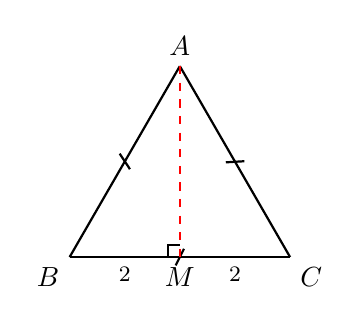
\begin{tikzpicture}[scale=0.7, thick,
  tickone/.style={postaction={decorate, decoration={markings,
    mark=at position 0.5 with {\draw (-1.5pt,-3pt) -- (1.5pt,3pt);}}}}]
  \coordinate (B) at (0,0);
  \coordinate (C) at (4,0);
  \coordinate (A) at (2, {2*sqrt(3)});
  \coordinate (M) at (2,0);
  \draw[tickone] (A) -- (B);
  \draw[tickone] (B) -- (C);
  \draw[tickone] (C) -- (A);
  \draw[red, dashed] (A) -- (M);
  % 直角
  \draw (1.78,0) -- (1.78,0.22) -- (2,0.22);
  \node[below left] at (B) {$B$};
  \node[below right] at (C) {$C$};
  \node[above] at (A) {$A$};
  \node[below] at (M) {$M$};
  \node[font=\footnotesize, below] at (1,0) {$2$};
  \node[font=\footnotesize, below] at (3,0) {$2$};
\end{tikzpicture}
\end{document}
